\documentclass{article} % For LaTeX2e
\usepackage{nips13submit_e,times}
\usepackage{hyperref}
\usepackage{url}
\usepackage{graphicx}
\usepackage{amsmath}
\usepackage{amsfonts}
\usepackage{upgreek}
\usepackage{subfigure}
\usepackage{algorithm}
\usepackage{placeins}
\usepackage{algpseudocode}
\usepackage{tkz-graph}
\usetikzlibrary{arrows}
%\usepackage{amsmath}
%\usepackage{amssymb}
%\usepackage{package}
%\usepackage{graphicx}
%\usepackage[utf8]{inputenc}  
%\usepackage[T1]{fontenc} 
%\usepackage[top=1cm,bottom=1cm,left=0.5cm,right=1.5cm,asymmetric]{geometry}
%\usepackage{amsfonts}
%\usepackage{graphicx}
%\usepackage{amsmath}
%\usepackage{caption}
%\usepackage{subcaption}
%\usepackage{float}
%\usepackage{subfig}
%\usepackage{fancyhdr}
%\documentstyle[nips13submit_09,times,art10]{article} % For LaTeX 2.09


\title{Significant perturbations in observability graph}

\author{
Oussama Ennafii\\
Master MVA\\
ENS Cachan\\
\texttt{oennafii@ens-cachan.fr} \\
\And
Sammy Khalife \\
Master MVA\\
ENS Cachan\\
\texttt{skhalife@ens-cachan.fr}
}

% The \author macro works with any number of authors. There are two commands
% used to separate the names and addresses of multiple authors: \And and \AND.
%
% Using \And between authors leaves it to \LaTeX{} to determine where to break
% the lines. Using \AND forces a linebreak at that point. So, if \LaTeX{}
% puts 3 of 4 authors names on the first line, and the last on the second
% line, try using \AND instead of \And before the third author name.

\newcommand{\fix}{\marginpar{FIX}}
\newcommand{\new}{\marginpar{NEW}}

%\nipsfinalcopy % Uncomment for camera-ready version
\bibliographystyle{plain}
\begin{document}


\maketitle

\begin{abstract}
Following the work on Online Learning with feedback graphs \cite{journals/corr/AlonCDK15} ,
we investigate the case of unstable graphs (even a small change in the graph structure like deleting or adding one edge can change the regret of the algorithm significantly), and design experiments which show the difference of the regret of the original and perturbed graph.
\end{abstract}

\section*{1 Introduction}
Given a feedback graph of observation, and a sequence of losses $(l_t)_{1 \leq t \leq T}$, let us denote $S$ the set of all strategies which have as output the sequence of actions $(I_t)_{1 \leq t \leq T}$. We denote the minimax regret by 
$$ R(G,T)=\min_{S} \max_{l_1,...,l_T} \mathbb{E}  \sum_{t=1}^{T} l_t(I_t) -\min_{i} \sum_{t=1}^{T}l_t(i)  $$
Which represents the best strategy answer to the worst case scenario in terms of loss sequence.
In [1], this minimax regret has been shown to be bounded with respect to the geometry of the feedback graph.~\\
~\\
If the graph is strongly observable with independence number $\alpha$, then 
$ R(G,T) = \tilde{\Uptheta}(\alpha^{1/2}T^{1/2})$.
If the graph is weakly observable with domination number $\delta$, then 
$ R(G,T) = \tilde{\Uptheta}(\delta^{1/2}T^{1/2})$
If the graph is unobservable, then 
$ R(G,T) = \tilde{\Uptheta}(T) $.

Similar to the EXP3 in the contex of adversarial bandits, the EXP3G algorithm [1] explores the graph given an exploration set U, an exploration rate $\gamma \in [0,1]$ and a learning rate $\eta > 0$. U(V) is the uniform distribution over V.\\

 \FloatBarrier
 \begin{algorithm}
 	\caption{EXP3G algorithm}\label{RS}
 	for t=1,...,T ~\\
 	Draw $ I_t \sim p_t = (1-\gamma)q_t + \gamma u(V) $ ~\\
 	Incure loss $l_t(I_t)$ and with respect to the feedback graph, observe $\{(i,l_t(i)), i \in N^{out}(I_t)\}$ ~\\
 	Update estimators and distribution :
 	$\hat{l}_{t}(i)=\frac{l_t(i)}{P_{t}(i)} \textbf{1}_{\{ i \in N^{out}(I_t)\}} \qquad$ $P_t(i)=\sum_{j \in N^{in}(i)}p_{t}(j)$, 
 	$q_{t+1}(i)=\frac{q_t(i)exp(-\eta \hat{l}_{t}(i))}{\sum_{j \in V}q_t{j}exp(-\eta \hat{l}_{j}(i))}$~\\
 	end
 \end{algorithm}
 \FloatBarrier
 
<<<<<<< HEAD
 %EXP3 and EWF
 As a reminder, the following feedback graphs gives the EWF and EXP3 framework, where respectively, we have full information on all the losses and EXP3 algorithm where we have information only on the chosen action.
 
 \begin{figure}[h]
 	
 	\subfigure[EWF framework]{
 		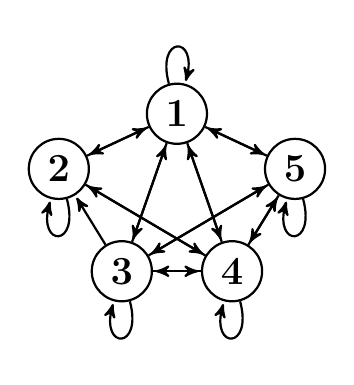
\begin{tikzpicture}[->,>=stealth',shorten >=1pt,auto,node distance=3cm,
 		thick,main node/.style={circle,draw,font=\Large\bfseries}]
 		\node[main node] (1) at (0,0) {1};
 		\node[main node] (2) at (-1.5,-0.7) {2};
 		\node[main node] (3) at (-0.7, -2) {3};
 		\node[main node] (4) at (0.7,-2) {4};
 		\node[main node] (5) at (1.5,-0.7) {5};
 		\path
 		(1) edge [loop above] node {} (1);
 		\path
 		(2) edge [loop below] node {} (2);
 		\path
 		(3) edge [loop below] node {} (3);
 		\path
 		(4) edge [loop below] node {} (4);
 		\path
 		(5) edge [loop below] node {} (5);
 
		  \tikzstyle{LabelStyle}=[fill=white,sloped]
		  %\tikzstyle{EdgeStyle}=[bend left]
		  \Edge[](1)(2)
		  \Edge[](1)(3)
		  \Edge[](1)(4)
		  \Edge[](1)(5)
		  \Edge[](2)(4)
 		  \Edge[](4)(3)
 		  \Edge[](5)(4)
 		  \Edge[](5)(3)
		  %\tikzstyle{EdgeStyle}=[bend right]
		  \Edge[](5)(1)
		  \Edge[](4)(1)
		  \Edge[](3)(2)
		  \Edge[](4)(2)
		  \Edge[](3)(4)
		  \Edge[](4)(5)
		  \Edge[](3)(1)
		  \Edge[](3)(5)
		  \Edge[](2)(1)
 		
 		\end{tikzpicture} }
 	\hfill
 	\subfigure[EXP3 framework]{
 			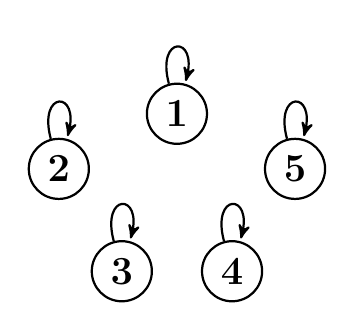
\begin{tikzpicture}[->,>=stealth',shorten >=1pt,auto,node distance=3cm,
 			thick,main node/.style={circle,draw,font=\Large\bfseries}]
 			\node[main node] (1) at (0,0) {1};
 			\node[main node] (2) at (-1.5,-0.7) {2};
 			\node[main node] (3) at (-0.7, -2) {3};
 			\node[main node] (4) at (0.7,-2) {4};
 			\node[main node] (5) at (1.5,-0.7) {5};
 			\path
 			(1) edge [loop above] node {} (1);
 			\path
 			(2) edge [loop above] node {} (2);
 			\path
 			(3) edge [loop above] node {} (3);
 			\path
 			(4) edge [loop above] node {} (4);
 			\path
 			(5) edge [loop above] node {} (5);

 			
 			\end{tikzpicture}
 			}
 \end{figure}
 
 
 
 
 
 
 
 
 
 
=======
 The goal of this project is to characterize unstable graphs. Unstable in this context means that if we add or delete an edge on the graph the regret behaviour will change dramatically. The main idea is to prove that the graphs on the edge between the three previous classes and to devise experiments showing this behaviour.
>>>>>>> dbf16d4bc630f7690e7382cebd559f3011fae7a6
 
\section*{2 Unstable graphs}
~\\
The goal of this section is to identify unstable graphs. Without loss of generality, we investigate the effect of adding one edge to a graph on the independence and weak domination numbers. Starting with the first case, the independence number is by definition the size of the largest independant set i.e. a set of vertices that are not connected by edges. Adding an edge to the graph measn that we connect two vertices that were not connected before. There are three cases. In the first one, the two newly connected vertices were part of a non maximal independent set, which means that the independence number is unchanged. The second case, is where there are more than one maximal independent set, which means aslo that the independence number remains unchanged. The last case, is when, at least, one of the vertices is part od the unique maximal independent set. In this case, the independence number is reduced by either one or two. In sumury, adding on edge to a graph means that the independence number varyies(diminishes) by $2$ at the maximum. Reciprocally, deleting an edge wil have the reverse effect.\\

Concerning the weak domination number, we start by identifying three possible cases. In the first one, we add an edge connecting going to a non observable vertice. In that case, this vertice becomes a weakly observable and all dominating sets would incorporate the dominating vertice - if it is not already in - which means that the weak domination number is at most augmented by $1$. If the new edge goes to a weakly observable vertice, the minimal dominating set would be unchanged because there exists an other dominating vertice ithat is already being accounted for. In the case where it is a strongly observable the dominating sets are all unchanged. So, in a nutshell, the weak domination number varyies at most by $1$. Reciprocally, deleting an edge wil have the reverse effect.\\

Based on the previous reasoning and the Theorem $1$ in \cite{journals/corr/AlonCDK15}, if the graph stays in the same class after adding or deleting a graph the bounds on regrets do not change by much and more importantly it does not change its evolution with respect to the time evolution.\\

Now we need to investigate the cases were graphs goes from one class to another by just adding or deleting an edge. There are three possibilities at hand: going from a strongly observable graphs to weakly observable onesa , going from the strong observable graph to an non observable one and going from a weakly observable graph to a non observable one ; and vice versa.\\

 Let's start with a strongly observable graph. We can subdivise the set of vertices $V$  into four sets: $V_1$ the set of vertices$i$ such that  $i \notin N^{in}(i)$, $V_2$ the set of vertices$i$ such that  $i \in N^{in}(i) \text{ and } \vert N^{in}(i)\vert=\vert V \vert$, $V_3$ the set of vertices$i$ such that  $i \in N^{in}(i) \text{ and } \vert N^{in}(i)\vert=1$ and $V_4$ the set of vertices$i$ such that  $i \in N^{in}(i) \text{ and } 1<\vert N^{in}(i)\vert<\vert V \vert$. Adding an edge to such a graph would certainly not make it changing its nature, so we will focus on the effect of deleting an edge. If we delete an edge going to a vertice in $V_2$, this vertice would stay strongly observable in any case, whereas if it is in $V_1$ this means that deleting any edge going to the vertice would make it weakly observable. If we consider now a vertice in $V_3$ deleting the only edge which was a self loop will make the vertice and the graph unobservable. In the other hand two cases are identified: the first one is when we delete the self loop, in that case we get a weakly obserable vertice or we delete an other incoming edge wich changes nothing to the nature\\
  of the graph. In sumury, if $V_2= \emptyset$ and we delete an incoming edge for a vertice in $V_1$ or the self loop for a vertice in $V_4$, we would get a weakly observable graph. If we maintain  $V_2= \emptyset$, $V_3 \neq \emptyset$ and we delete the self loop for a vertice in $V_3$, we get a non observable graph. This is the only way to go to a non observable or a weakly observable graph from a strongly observable one by deleting one edge and vice versa.\\
  
  We consider now the weakly observable graph and we subdivise the set of vertices $V$ into two sets this time:$V_5$ where vertices $i$ have only one incoming edge and $V_6$ where vertices $i$ have more than one incoming edge. We are interested into getting a non observable graph by deleting only one edge. If we delete an incoming edge for a vertice in $V_6$ it remains observable while if we do the same thing to a vertice in $V_5$ the vertice becomes non observable. And thus, the only way to get a a non observable graph from a weakly observable one by deleting only one edge, is to have $V_5 \neq \emptyset$ and to delete an incoming edge of a vertice in that set.\\
  
  There are a  lot of unstable graphs to be considered, so we need to investigate the graphs that can yield the most difference possible. There is only one case to consider here since the bound on the non observable case depend only on $T$ the time horizon. So we are looking for a graph that can yield too different independence and weak domination numbers. We start from a strongly observable set. the weak domination number of the resulting graph after deleting an edge is obviously $\delta=1$ since there is only one weakly observable vertice. So that leaves us with one choice. getting the independence number $\alpha$ the bigger possible. The bandit graph is the only graph to have $\alpha =\vert V\vert$ but we cannot get a weakly observable graph by only deleting one edge. So the best we can do is to have $\alpha=\vert V \vert -1$. To get an example, we can just add one edge to the bandit graph and delet the self loop on the vertice with an incoming edge. We can add an edge coming from the same vertice from where originates the previous edge and going to another vertice. We continue doing it until we get the graph in figure ~\ref{fig::ex} . All of these, graphs has an $\alpha= \vert V\vert -1$. An obvious choice would be then to get a graph as big as possible so as to get a big difference between $\alpha$ and $\delta$
~\\
\section*{3 Experiments }




\SetVertexNormal[Shape      = circle,
FillColor  = white,
LineWidth  = 2pt]
\SetUpEdge[lw         = 1.5pt,
color      = black,
labelcolor = white,
labeltext  = red,
labelstyle = {sloped,draw,text=blue}]


\begin{figure}[h]
	
<<<<<<< HEAD
\subfigure[Unpertubed, strongly observable $\alpha=4$]{
=======
\subfigure[\label{fig::ex}before]{
>>>>>>> dbf16d4bc630f7690e7382cebd559f3011fae7a6
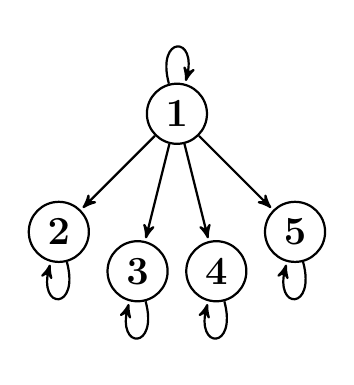
\begin{tikzpicture}[->,>=stealth',shorten >=1pt,auto,node distance=3cm,
thick,main node/.style={circle,draw,font=\Large\bfseries}]
\node[main node] (1) at (0,0) {1};
\node[main node] (2) at (-1.5,-1.5) {2};
\node[main node] (3) at (-0.5, -2) {3};
\node[main node] (4) at (0.5,-2) {4};
\node[main node] (5) at (1.5,-1.5) {5};
\path
(1) edge [loop above] node {} (1);
\path
(2) edge [loop below] node {} (2);
\path
(3) edge [loop below] node {} (3);
\path
(4) edge [loop below] node {} (4);
\path
(5) edge [loop below] node {} (5);
%edge [bend right] node {0.4} (2)
%(1) edge node [below]{} (2)
%%(1) edge [loop below] node {} (3)
%%edge node[right] {0.1} (1)
%(1) edge node[below] {} (3); 
%(1) edge node[below] {} (4);
%(1) edge node[below] {} (5);    
\draw (1) -- (2);
\draw (1) -- (3);
\draw (1) -- (4);
\draw (1) -- (5); 
\end{tikzpicture} }

\subfigure[Pertubed (weakly observable), $\delta=1$]{
	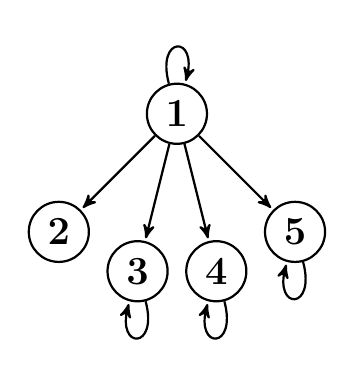
\begin{tikzpicture}[->,>=stealth',shorten >=1pt,auto,node distance=3cm,
	thick,main node/.style={circle,draw,font=\Large\bfseries}]
	
	\node[main node] (1) at (0,0) {1};
	\node[main node] (2) at (-1.5,-1.5) {2};
	\node[main node] (3) at (-0.5, -2) {3};
	\node[main node] (4) at (0.5,-2) {4};
	\node[main node] (5) at (1.5,-1.5) {5};
	\path
	(1) edge [loop above] node {} (1);
	%\path
	%(2) edge [loop below] node {} (2);
	\path
	(3) edge [loop below] node {} (3);
	\path
	(4) edge [loop below] node {} (4);
	\path
	(5) edge [loop below] node {} (5);
	%edge [bend right] node {0.4} (2)
	%(1) edge node [below]{} (2)
	%%(1) edge [loop below] node {} (3)
	%%edge node[right] {0.1} (1)
	%(1) edge node[below] {} (3); 
	%(1) edge node[below] {} (4);
	%(1) edge node[below] {} (5);    
	\draw (1) -- (2);
	\draw (1) -- (3);
	\draw (1) -- (4);
	\draw (1) -- (5);
	\end{tikzpicture} }

\subfigure[Pertubed (non observable)]{
	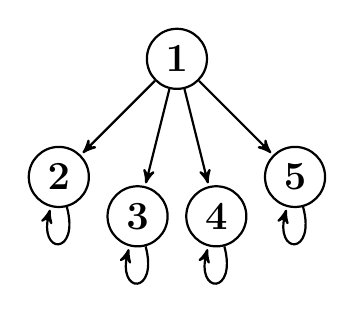
\begin{tikzpicture}[->,>=stealth',shorten >=1pt,auto,node distance=3cm,
	thick,main node/.style={circle,draw,font=\Large\bfseries}]
	
	\node[main node] (1) at (0,0) {1};
	\node[main node] (2) at (-1.5,-1.5) {2};
	\node[main node] (3) at (-0.5, -2) {3};
	\node[main node] (4) at (0.5,-2) {4};
	\node[main node] (5) at (1.5,-1.5) {5};
	%\path
	%(1) edge [loop above] node {} (1);
	\path
	(2) edge [loop below] node {} (2);
	\path
	(3) edge [loop below] node {} (3);
	\path
	(4) edge [loop below] node {} (4);
	\path
	(5) edge [loop below] node {} (5);
	%edge [bend right] node {0.4} (2)
	%(1) edge node [below]{} (2)
	%%(1) edge [loop below] node {} (3)
	%%edge node[right] {0.1} (1)
	%(1) edge node[below] {} (3); 
	%(1) edge node[below] {} (4);
	%(1) edge node[below] {} (5);    
	\draw (1) -- (2);
	\draw (1) -- (3);
	\draw (1) -- (4);
	\draw (1) -- (5);
\end{tikzpicture} }
\hfill
\subfigure[Associated worst case regret]{
	\includegraphics[width=5cm]{nonobservable.jpg}
}
\end{figure}
%\caption{Revealing action graph (strongly observable)} \label{fig:M1}







\bibliography{references.bib}

\end{document}
